% header.tex -- Beamer preamble for ECON 692 (Spring 2026)
% Compile with XeLaTeX

\documentclass[aspectratio=169, 12pt]{beamer}

% ── Theme ──────────────────────────────────────────────
\usetheme{default}
\usecolortheme{default}
\setbeamertemplate{navigation symbols}{}
\setbeamertemplate{footline}[frame number]

% ── Colors ─────────────────────────────────────────────
\definecolor{usfgreen}{HTML}{00543C}
\definecolor{usfgold}{HTML}{FDBB30}
\definecolor{lightgray}{HTML}{F5F5F5}
\definecolor{codebg}{HTML}{F0F0F0}
\definecolor{darkgray}{HTML}{333333}

\setbeamercolor{title}{fg=usfgreen}
\setbeamercolor{frametitle}{fg=usfgreen}
\setbeamercolor{structure}{fg=usfgreen}
\setbeamercolor{normal text}{fg=darkgray}
\setbeamercolor{itemize item}{fg=usfgreen}
\setbeamercolor{itemize subitem}{fg=usfgreen!80}
\setbeamercolor{itemize subsubitem}{fg=usfgreen!60}
\setbeamercolor{block title}{bg=usfgreen, fg=white}
\setbeamercolor{block body}{bg=lightgray}
\setbeamercolor{footline}{fg=gray}

% ── Fonts ──────────────────────────────────────────────
\usepackage{fontspec}
\setsansfont{Helvetica Neue}[
  BoldFont = {Helvetica Neue Bold},
  ItalicFont = {Helvetica Neue Italic},
]
\setmonofont{Menlo}[Scale=0.85]

% ── Beamer fonts ───────────────────────────────────────
\setbeamerfont{title}{size=\LARGE, series=\bfseries}
\setbeamerfont{subtitle}{size=\large}
\setbeamerfont{frametitle}{size=\Large, series=\bfseries}
\setbeamerfont{framesubtitle}{size=\normalsize}
\setbeamerfont{footline}{size=\tiny}

% ── Frame title formatting ─────────────────────────────
\setbeamertemplate{frametitle}{%
  \vskip6pt%
  \insertframetitle%
  \ifx\insertframesubtitle\empty\else%
    \\[2pt]{\usebeamerfont{framesubtitle}\usebeamercolor[fg]{framesubtitle}\insertframesubtitle}%
  \fi%
  \vskip2pt%
  {\color{usfgreen}\hrule height 1.5pt}%
  \vskip4pt%
}

% ── Title page ─────────────────────────────────────────
\setbeamertemplate{title page}{
  \vfill
  \begin{center}
    {\usebeamerfont{title}\usebeamercolor[fg]{title}\inserttitle}\\[8pt]
    \ifx\insertsubtitle\empty\else
      {\usebeamerfont{subtitle}\usebeamercolor[fg]{subtitle}\insertsubtitle}\\[12pt]
    \fi
    {\color{usfgreen}\rule{0.4\textwidth}{1.5pt}}\\[12pt]
    {\normalsize\insertauthor}\\[4pt]
    {\small\insertinstitute}\\[4pt]
    {\small\insertdate}
  \end{center}
  \vfill
}

% ── Packages ───────────────────────────────────────────
\usepackage{amsmath, amssymb}
\usepackage{graphicx}
\usepackage{tikz}
\usepackage{array}
\usepackage{booktabs}
\usepackage{hyperref}
\hypersetup{colorlinks=true, linkcolor=usfgreen, urlcolor=usfgreen!80}

% ── Code listings ──────────────────────────────────────
\usepackage{listings}
\lstset{
  basicstyle=\ttfamily\small,
  backgroundcolor=\color{codebg},
  frame=single,
  framerule=0pt,
  framexleftmargin=4pt,
  framexrightmargin=4pt,
  framextopmargin=4pt,
  framexbottommargin=4pt,
  breaklines=true,
  showstringspaces=false,
  columns=fullflexible,
  keepspaces=true,
  literate={~}{{\textasciitilde}}1,
}

\lstdefinestyle{terminal}{
  basicstyle=\ttfamily\small\color{darkgray},
  backgroundcolor=\color{codebg},
  language=bash,
}

% ── Itemize bullets ────────────────────────────────────
\setbeamertemplate{itemize item}{\small\raise1pt\hbox{\textbullet}}
\setbeamertemplate{itemize subitem}{\small\raise1pt\hbox{--}}
\setbeamertemplate{itemize subsubitem}{\small\raise1pt\hbox{$\cdot$}}

% ── Useful macros ──────────────────────────────────────
\newcommand{\E}{\mathbb{E}}
\newcommand{\Var}{\mathrm{Var}}
\newcommand{\indep}{\perp\!\!\!\perp}

% ── Section pages ──────────────────────────────────────
\AtBeginSection[]{
  \begin{frame}
    \vfill
    \centering
    {\Large\bfseries\color{usfgreen}\insertsectionhead}
    \vfill
  \end{frame}
}


\title{Empirical Strategy \& Project Setup}
\subtitle{ECON 692 -- Applied Economics Seminar}
\author{Andrew Hobbs}
\institute{University of San Francisco}
\date{February 12, 2026}

\begin{document}

% ══════════════════════════════════════════════════════════
%  SECTION 1: Welcome & Agenda
% ══════════════════════════════════════════════════════════

\begin{frame}[plain]
  \titlepage
\end{frame}

\begin{frame}{Today's Agenda}
  \begin{tabular}{@{}r@{\hspace{8pt}}l@{\hspace{16pt}}l@{}}
    \toprule
    \textbf{Time} & \textbf{Duration} & \textbf{Activity} \\
    \midrule
    4:35 & 5 min  & Welcome \& check-in \\
    4:40 & 30 min & Methods overview: DiD, SC, SDID \\
    5:10 & 30 min & Empirical strategy workshop \\
    5:40 & 10 min & Break \\
    5:50 & 40 min & Git \& GitHub setup \\
    6:30 & 10 min & Break \\
    6:40 & 60 min & Data sprint: initial code \& results \\
    7:40 & 30 min & Lightning presentations \\
    8:10 & 5 min  & Wrap-up \\
    \bottomrule
  \end{tabular}
\end{frame}

\begin{frame}{Check-in}
  \begin{itemize}
    \item How did proposals go? Any surprises?
    \item Has anyone changed their topic since last week?
    \item Where are you on finding data?
  \end{itemize}
  \vspace{12pt}
  \begin{block}{Reminder}
    Data Report is due \textbf{Friday, February 20} at 11:59pm.
  \end{block}
\end{frame}

% ══════════════════════════════════════════════════════════
%  SECTION 2: Methods Overview
% ══════════════════════════════════════════════════════════

\section{Methods Overview}

\begin{frame}{The Identification Problem}
  You have a research question and data. How do you \textbf{identify a causal effect}?

  \vspace{12pt}

  \begin{itemize}
    \item Last week: potential outcomes, ATE, selection bias
    \item Today: three methods for \textbf{panel data} settings where treatment varies across units and time
    \begin{itemize}
      \item Difference-in-Differences (DiD)
      \item Synthetic Control (SC)
      \item Synthetic Difference-in-Differences (SDID)
    \end{itemize}
    \item Focus: \textbf{key assumptions} and \textbf{when to use each}
  \end{itemize}
\end{frame}

% ── Difference-in-Differences ──────────────────────────

\begin{frame}{Difference-in-Differences: Setup}
  \textbf{Setting:} Panel data with two groups and two periods.

  \vspace{4pt}

  \begin{columns}[T]
    \begin{column}{0.45\textwidth}
      \centering
      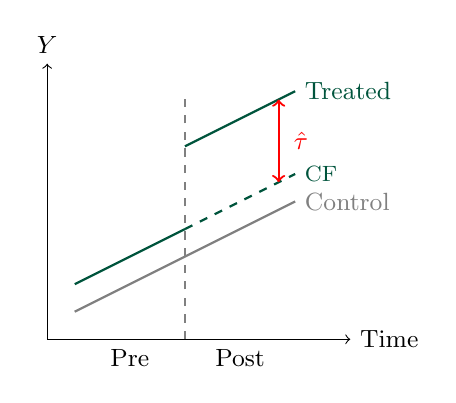
\begin{tikzpicture}[scale=0.7]
        % Axes
        \draw[->] (0,0) -- (5.5,0) node[right] {\small Time};
        \draw[->] (0,0) -- (0,5) node[above] {\small $Y$};
        % Treatment line
        \draw[thick, usfgreen] (0.5,1) -- (2.5,2);
        \draw[thick, usfgreen] (2.5,3.5) -- (4.5,4.5);
        % Counterfactual
        \draw[thick, usfgreen, dashed] (2.5,2) -- (4.5,3);
        \node[usfgreen, right, font=\footnotesize] at (4.5,3) {CF};
        % Control line
        \draw[thick, gray] (0.5,0.5) -- (2.5,1.5) -- (4.5,2.5);
        % Treatment effect
        \draw[<->, red, thick] (4.2,2.85) -- (4.2,4.35);
        \node[right, red] at (4.3,3.6) {\small $\hat{\tau}$};
        % Labels
        \node[usfgreen, right] at (4.5,4.5) {\small Treated};
        \node[gray, right] at (4.5,2.5) {\small Control};
        % Vertical line
        \draw[dashed, gray] (2.5,0) -- (2.5,4.5);
        \node[below] at (1.5,0) {\small Pre};
        \node[below] at (3.5,0) {\small Post};
      \end{tikzpicture}
    \end{column}

    \begin{column}{0.52\textwidth}
      \begin{itemize}
        \item \textbf{Treatment group}: affected by policy/event
        \item \textbf{Control group}: not affected
        \item \textbf{Pre-period}: before treatment
        \item \textbf{Post-period}: after treatment
      \end{itemize}
    \end{column}
  \end{columns}

  \vspace{2pt}
  The DiD estimator:\quad
  $\hat{\tau}^{\text{did}} = (\bar{Y}_{T,\text{post}} - \bar{Y}_{T,\text{pre}}) - (\bar{Y}_{C,\text{post}} - \bar{Y}_{C,\text{pre}})$
\end{frame}

\begin{frame}{DiD: A Simple Example}
  Suppose New Jersey raises its minimum wage in 1992. Pennsylvania does not.

  \vspace{8pt}

  \begin{tabular}{@{}lccc@{}}
    \toprule
    & \textbf{Before} & \textbf{After} & \textbf{Change} \\
    \midrule
    NJ (treated)    & 20.4 FTE & 21.0 FTE & $+0.6$ \\
    PA (control)    & 23.3 FTE & 21.2 FTE & $-2.1$ \\
    \midrule
    \textbf{DiD}    &          &          & $0.6 - (-2.1) = \mathbf{+2.7}$ \\
    \bottomrule
  \end{tabular}

  \vspace{8pt}

  \begin{itemize}
    \item NJ employment \textit{rose} relative to PA after the minimum wage increase
    \item DiD estimate: $+2.7$ FTE employees per restaurant (Card \& Krueger, 1994)
    \item \textit{For your project:} think about what fills each cell of this table
  \end{itemize}
\end{frame}

\begin{frame}{DiD: Key Assumption}
  \begin{block}{Parallel Trends Assumption}
    In the absence of treatment, the treatment and control groups would have followed the \textbf{same trajectory} over time.
  \end{block}

  \vspace{8pt}

  \begin{itemize}
    \item This is \textbf{untestable} -- we can never observe the counterfactual
    \item But we can check: did trends look parallel \textit{before} treatment?
    \item Common to show a pre-trends plot as supporting evidence
  \end{itemize}

  \vspace{8pt}

  \textit{For your project: what event or trend could violate parallel trends?}
\end{frame}

\begin{frame}{DiD: Staggered Treatment}
  \textbf{Caution:} With staggered treatment adoption (units treated at different times), na\"ive two-way fixed effects (TWFE) regression can give \textbf{biased} estimates.

  \vspace{8pt}

  \begin{itemize}
    \item Already-treated units can act as ``controls'' -- biases estimates
    \item Effects can be heterogeneous across timing groups
    \item Modern solutions handle this correctly:
    \begin{itemize}
      \item \texttt{did} package (Callaway \& Sant'Anna)
      \item \texttt{fixest::sunab()} (Sun \& Abraham)
    \end{itemize}
  \end{itemize}

  \vspace{8pt}

  If your treatment rolls out at different times, use one of these packages instead of basic TWFE.
\end{frame}

\begin{frame}{DiD: When to Use It}
  \textbf{DiD is a good fit when you have:}
  \begin{itemize}
    \item A clear treatment/control group distinction
    \item Pre- and post-treatment observations for both groups
    \item Reasonable parallel trends argument
    \item A \textbf{substantial number} of treated and control units
  \end{itemize}

  \vspace{8pt}

  \textbf{Packages:}
  \begin{itemize}
    \item R: \texttt{fixest}, \texttt{did}, \texttt{DIDmultiplegt}
    \item Python: \texttt{pyfixest}, \texttt{linearmodels}
  \end{itemize}
\end{frame}

% ── Synthetic Control ──────────────────────────────────

\begin{frame}{Synthetic Control: Setup}
  \textbf{Setting:} A single (or few) treated unit(s), many potential controls.

  \vspace{6pt}

  \begin{columns}[T]
    \begin{column}{0.45\textwidth}
      \centering
      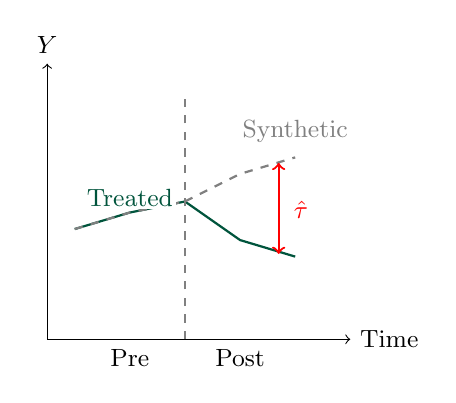
\begin{tikzpicture}[scale=0.7]
        % Axes
        \draw[->] (0,0) -- (5.5,0) node[right] {\small Time};
        \draw[->] (0,0) -- (0,5) node[above] {\small $Y$};
        % Treated (solid)
        \draw[thick, usfgreen] (0.5,2) -- (1.5,2.3) -- (2.5,2.5);
        \draw[thick, usfgreen] (2.5,2.5) -- (3.5,1.8) -- (4.5,1.5);
        % Synthetic control
        \draw[thick, gray, dashed] (0.5,2) -- (1.5,2.3) -- (2.5,2.5);
        \draw[thick, gray, dashed] (2.5,2.5) -- (3.5,3.0) -- (4.5,3.3);
        % Treatment effect
        \draw[<->, red, thick] (4.2,1.55) -- (4.2,3.2);
        \node[right, red] at (4.3,2.35) {\small $\hat{\tau}$};
        % Labels
        \node[usfgreen, above, fill=white, inner sep=1pt] at (1.5,2.35) {\small Treated};
        \node[gray, above] at (4.5,3.4) {\small Synthetic};
        % Vertical line
        \draw[dashed, gray] (2.5,0) -- (2.5,4.5);
        \node[below] at (1.5,0) {\small Pre};
        \node[below] at (3.5,0) {\small Post};
      \end{tikzpicture}
    \end{column}

    \begin{column}{0.52\textwidth}
      \begin{itemize}
        \item \textbf{Treated unit}: e.g., California, Germany
        \item \textbf{Donor pool}: untreated units (other states, countries)
        \item Construct a \textbf{weighted combination} of donors that matches the treated unit's \textit{pre-treatment} trajectory
        \item Treatment effect = gap between treated and synthetic after treatment
      \end{itemize}
    \end{column}
  \end{columns}
\end{frame}

\begin{frame}{SC: Key Requirements}
  From Abadie (2021), practical requirements for synthetic controls:

  \vspace{8pt}

  \begin{enumerate}
    \item \textbf{Sizable donor pool} of untreated units
    \item \textbf{Long pre-treatment period} to achieve good match
    \item \textbf{No spillovers}: treatment of one unit should not affect donors
    \item \textbf{Convex hull}: treated unit's characteristics should be within the range of the donor pool (no extrapolation) -- \textit{relaxed by augmented SC}
    \item Treatment is at an \textbf{aggregate level} (state, country, region)
  \end{enumerate}

  \vspace{8pt}

  \textit{Does your setting have enough untreated units to build a donor pool?}

  \vspace{4pt}

  \textbf{Packages:}
  \begin{itemize}
    \item R: \texttt{Synth}, \texttt{tidysynth}, \texttt{augsynth} (ridge-augmented; allows extrapolation beyond convex hull)
  \end{itemize}
\end{frame}

% ── SDID ───────────────────────────────────────────────

\begin{frame}{Synthetic Difference-in-Differences}
  \small
  Arkhangelsky, Athey, Hirshberg, Imbens, and Wager (2021):

  \vspace{2pt}

  \begin{columns}[T]
    \begin{column}{0.35\textwidth}
      \centering
      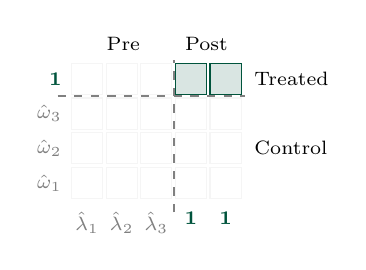
\begin{tikzpicture}[scale=0.44, font=\scriptsize]
        % Grid
        \foreach \y in {0,...,3} {
          \foreach \x in {0,...,4} {
            \draw[lightgray, fill=white] (\x,\y) rectangle +(0.9,0.9);
          }
        }
        % Treated unit (top row) - post period highlighted
        \draw[usfgreen, fill=usfgreen!15] (3,3) rectangle +(0.9,0.9);
        \draw[usfgreen, fill=usfgreen!15] (4,3) rectangle +(0.9,0.9);
        % Unit weights (left side)
        \node[left, usfgreen] at (0,3.45) {\textbf{1}};
        \node[left, gray] at (0,2.45) {$\hat{\omega}_3$};
        \node[left, gray] at (0,1.45) {$\hat{\omega}_2$};
        \node[left, gray] at (0,0.45) {$\hat{\omega}_1$};
        % Time weights (bottom)
        \node[below, gray] at (0.45,-0.1) {$\hat{\lambda}_1$};
        \node[below, gray] at (1.45,-0.1) {$\hat{\lambda}_2$};
        \node[below, gray] at (2.45,-0.1) {$\hat{\lambda}_3$};
        \node[below, usfgreen] at (3.45,-0.1) {\textbf{1}};
        \node[below, usfgreen] at (4.45,-0.1) {\textbf{1}};
        % Divider
        \draw[dashed, gray, thick] (2.95,-0.4) -- (2.95,4);
        \node[above] at (1.5,4) {Pre};
        \node[above] at (3.9,4) {Post};
        \draw[dashed, gray, thick] (-0.4,2.95) -- (5,2.95);
        \node[right] at (5,3.45) {Treated};
        \node[right] at (5,1.45) {Control};
      \end{tikzpicture}

    \end{column}

    \begin{column}{0.62\textwidth}
      \begin{itemize}
        \item Combines the best of DiD and SC
        \item Like SC: \textbf{unit weights} $\hat{\omega}$ reweight controls
        \item Novel: \textbf{time weights} $\hat{\lambda}$ emphasize informative pre-periods
        \item Like DiD: unit FEs, valid large-panel inference
      \end{itemize}

      \vspace{2pt}

      \textbf{Why SDID?} More robust than DiD when parallel trends is approximate; more robust than SC with few pre-periods.
      \textbf{Package:} R \texttt{synthdid}
    \end{column}
  \end{columns}
\end{frame}

\begin{frame}{Comparison}
  \footnotesize
  \begin{tabular}{@{}l>{\raggedright\arraybackslash}p{3.2cm}>{\raggedright\arraybackslash}p{3.2cm}>{\raggedright\arraybackslash}p{3.2cm}@{}}
    \toprule
    & \textbf{DiD} & \textbf{Synthetic Control} & \textbf{SDID} \\
    \midrule
    \textbf{Key assumption}
      & Parallel trends
      & Good pre-treatment fit; no spillovers
      & Weaker than both \\[4pt]
    \textbf{Best when}
      & Many treated \& control units
      & Few treated units, many controls
      & Either setting \\[4pt]
    \textbf{Limitations}
      & Biased with staggered treatment (na\"ive TWFE)
      & Needs long pre-period; single treated unit
      & Newer, less established \\[4pt]
    \textbf{R packages}
      & \texttt{fixest}, \texttt{did}
      & \texttt{Synth}, \texttt{augsynth}
      & \texttt{synthdid} \\
    \bottomrule
  \end{tabular}

  \vspace{6pt}

  \small
  \textit{Based on your data structure, which method seems most promising for your project?}
\end{frame}

\begin{frame}{Continuous Treatments: The Standard Approach}
  Many DiD applications involve treatments that are not simply on/off:
  \begin{itemize}
    \item Varying tax rates, pollution levels, subsidy amounts, minimum wages
    \item Distance to a facility, intensity of exposure to a policy
  \end{itemize}

  \vspace{8pt}

  \textbf{The standard approach} -- TWFE with a continuous dose variable:
  \[
    Y_{it} = \underbrace{\theta_t}_{\text{time FE}} + \underbrace{\eta_i}_{\text{unit FE}} + \beta^{twfe} \underbrace{D_i \cdot \text{Post}_t}_{\text{dose} \times \text{post}} + v_{it}
  \]

  \vspace{4pt}

  Researchers typically interpret $\beta^{twfe}$ as the ``effect of one more unit of treatment.''

  \vspace{4pt}

  \textit{But is this correct?}
\end{frame}

\begin{frame}{Continuous Treatments: The Problem}
  \textbf{The problem} (Callaway, Goodman-Bacon, \& Sant'Anna, 2024):

  \vspace{8pt}

  \begin{itemize}
    \item $\beta^{twfe}$ is a weighted average of dose-specific effects, but \textbf{weights can be negative}
    \item Even with non-negative weights, TWFE conflates two different things:
  \end{itemize}

  \vspace{6pt}

  \begin{columns}[T]
    \begin{column}{0.47\textwidth}
      \textbf{\textcolor{usfgreen}{Level effects}}\\[4pt]
      Does getting dose $d$ vs.\ 0 change outcomes?\\[4pt]
      \textit{Requires:} standard parallel trends
    \end{column}
    \begin{column}{0.47\textwidth}
      \textbf{\textcolor{usfgreen}{Causal responses}}\\[4pt]
      Does a marginal increase in dose change outcomes?\\[4pt]
      \textit{Requires:} strong parallel trends (restricts heterogeneity)
    \end{column}
  \end{columns}

  \vspace{8pt}

  These are \textit{different parameters} requiring \textit{different assumptions}. TWFE mixes them.
\end{frame}

\begin{frame}{Continuous Treatments: Solutions}
  \small
  \textbf{Two distinct causal parameters:}

  \footnotesize
  \begin{tabular}{@{}l>{\raggedright\arraybackslash}p{4.2cm}>{\raggedright\arraybackslash}p{4.2cm}@{}}
    \toprule
    & \textbf{Level effects}\newline (ATT at dose $d$) & \textbf{Causal responses}\newline (marginal effect) \\
    \midrule
    \textbf{Assumption} & Standard parallel trends (on untreated outcomes) & Strong parallel trends (restricts heterogeneity across doses) \\[3pt]
    \textbf{Compares} & Treated vs.\ untreated & Adjacent dose groups \\
    \bottomrule
  \end{tabular}

  \small
  \vspace{6pt}

  \textbf{Packages:}
  \begin{itemize}
    \item R: \texttt{contdid} (Callaway et al.) -- level effects and causal response curves as functions of dose
    \item de Chaisemartin et al.\ (2024) -- extends to \textbf{no stayers} (every unit's treatment changes); R/Stata: \texttt{did\_multiplegt\_stat}, \texttt{did\_multiplegt\_dyn}
  \end{itemize}

  \textbf{Bottom line:} Don't run TWFE with a continuous $D$. Use \texttt{contdid}.
\end{frame}

% ══════════════════════════════════════════════════════════
%  SECTION 3: Empirical Strategy Workshop
% ══════════════════════════════════════════════════════════

\section{Empirical Strategy Workshop}

\begin{frame}{What Is an Empirical Strategy?}
  Your empirical strategy is the \textbf{plan for answering your research question with data}.

  \vspace{8pt}

  Four components:
  \begin{enumerate}
    \item \textbf{Method}: Which estimation approach? (DiD, SC, SDID, OLS, IV, RDD, \ldots)
    \item \textbf{Data}: What variables, from where, at what level?
    \item \textbf{Identification}: What variation are you exploiting? Why is it credible?
    \item \textbf{Threats}: What could go wrong? How will you address it?
  \end{enumerate}
\end{frame}

\begin{frame}{Strategy Worksheet}
  Take 10 minutes. Write your answers on paper or in a document.

  \vspace{8pt}

  \begin{enumerate}
    \item What is your \textbf{treatment or intervention}?
    \item What is your main \textbf{outcome variable}?
    \item What is your \textbf{comparison/control group}?
    \item What \textbf{time periods} do you have data for?
    \item What are the main \textbf{threats to identification}?
    \item Which \textbf{method} fits your setting, and why?
  \end{enumerate}

  \vspace{8pt}

  \textbf{Goal:} Write a 1-paragraph empirical strategy statement.
\end{frame}

\begin{frame}{Choosing Packages}
  Once you have a method in mind, pick your tools:

  \vspace{8pt}

  \textbf{If using R:}
  \begin{itemize}
    \item DiD $\rightarrow$ \texttt{fixest} (fast, flexible), \texttt{did} (Callaway--Sant'Anna estimator)
    \item SC $\rightarrow$ \texttt{augsynth} (ridge-augmented SC), \texttt{tidysynth} (tidy interface to \texttt{Synth})
    \item SDID $\rightarrow$ \texttt{synthdid}
    \item General regression $\rightarrow$ \texttt{fixest}, \texttt{lfe}, \texttt{estimatr}
  \end{itemize}

  \vspace{6pt}

  \textbf{If using Python:}
  \begin{itemize}
    \item DiD $\rightarrow$ \texttt{pyfixest}, \texttt{linearmodels}
    \item SC $\rightarrow$ \texttt{SparseSC}, or call R from Python via \texttt{rpy2}
    \item General $\rightarrow$ \texttt{statsmodels}, \texttt{linearmodels}
  \end{itemize}

  \vspace{8pt}

  \textbf{Task:} Identify the specific package(s) you'll use. Install them today.
\end{frame}

\begin{frame}{Share with a Partner}
  In pairs, spend 10 minutes each:
  \begin{enumerate}
    \item Read your empirical strategy statement to your partner
    \item Partner asks:
    \begin{itemize}
      \item What is the biggest threat to your identification?
      \item Is there an alternative control group you could use?
      \item Does the parallel trends / no spillovers assumption seem reasonable?
    \end{itemize}
    \item Revise your statement based on feedback
  \end{enumerate}
\end{frame}

% ══════════════════════════════════════════════════════════
%  SECTION 4: Git & GitHub Setup
% ══════════════════════════════════════════════════════════

\section{Git \& GitHub Setup}

\begin{frame}{Why Version Control?}
  \begin{columns}[T]
    \begin{column}{0.48\textwidth}
      \textbf{Without version control:}
      \begin{itemize}
        \item \texttt{analysis\_v2\_final\_FINAL.R}
        \item ``Which version has the fix?''
        \item ``I accidentally deleted my code''
        \item Impossible to reproduce results from 3 months ago
      \end{itemize}
    \end{column}
    \begin{column}{0.48\textwidth}
      \textbf{With Git:}
      \begin{itemize}
        \item Complete history of every change
        \item Undo mistakes instantly
        \item Collaborate without overwriting
        \item \textbf{Portfolio for job applications}
      \end{itemize}
    \end{column}
  \end{columns}
\end{frame}

\begin{frame}{Git Concepts (Just Three Things)}
  \begin{enumerate}
    \item \textbf{Repository (repo)}: A folder that Git tracks.
      \begin{itemize}
        \item Every change you \textit{commit} is saved forever.
      \end{itemize}
    \item \textbf{Commit}: A snapshot of your project at a point in time.
      \begin{itemize}
        \item Like ``Save As'' but you keep \textit{all} previous saves.
        \item Each commit has a message describing what changed.
      \end{itemize}
    \item \textbf{Push / Pull}: Sync between your computer and GitHub.
      \begin{itemize}
        \item \textbf{Push}: upload your commits to GitHub.
        \item \textbf{Pull}: download changes from GitHub.
      \end{itemize}
  \end{enumerate}
\end{frame}

\begin{frame}[fragile]{Step 1: Install Git \& Configure}
  Open your terminal and check if Git is installed:

  \begin{lstlisting}[style=terminal]
git --version
  \end{lstlisting}

  If not installed: \textbf{Mac:} \texttt{xcode-select --install} \quad \textbf{Windows:} \url{https://git-scm.com}

  \vspace{8pt}

  Configure your identity (one-time setup):
  \begin{lstlisting}[style=terminal]
git config --global user.name "Your Name"
git config --global user.email "your.email@usfca.edu"
  \end{lstlisting}
\end{frame}

\begin{frame}{Step 2: GitHub Education}
  GitHub offers a free \textbf{Student Developer Pack}:
  \begin{itemize}
    \item Unlimited private repositories
    \item GitHub Copilot (AI code assistant)
    \item Free domain name and other tools
  \end{itemize}

  \vspace{8pt}

  \textbf{To sign up:}
  \begin{enumerate}
    \item Go to \url{https://github.com} -- create an account if you don't have one
    \item Visit \url{https://education.github.com/pack}
    \item Click ``Get your pack'' and verify with your \texttt{@usfca.edu} email
    \item Approval is usually instant or within a few hours
  \end{enumerate}

  \vspace{8pt}

  Do this now if you haven't already.
\end{frame}

\begin{frame}[fragile]{Step 3: Create a Repository on GitHub}
  \begin{enumerate}
    \item Go to \url{https://github.com} and click \textbf{``New repository''}
    \item Name it something descriptive: e.g., \texttt{econ692-capstone}
    \item Set it to \textbf{Private}
    \item Check \textbf{``Add a README file''}
    \item Check \textbf{``Add .gitignore''} and select the \texttt{R} or \texttt{Python} template
    \item Click \textbf{``Create repository''}
  \end{enumerate}
\end{frame}

\begin{frame}[fragile]{Step 4: Clone to Your Computer}
  On your repo page, click the green \textbf{``Code''} button and copy the URL.

  \vspace{8pt}

  In your terminal:
  \begin{lstlisting}[style=terminal]
cd ~/Documents  # or wherever you keep projects
git clone https://github.com/yourusername/econ692-capstone.git
cd econ692-capstone
  \end{lstlisting}

  \vspace{8pt}

  You now have a local copy of your repository.
\end{frame}

\begin{frame}[fragile]{Step 5: Project Structure}
  Create a clean folder structure for your project:

  \vspace{6pt}

  \begin{lstlisting}[style=terminal]
mkdir data code output paper
  \end{lstlisting}

  \vspace{6pt}

  \begin{tabular}{@{}ll@{}}
    \texttt{data/}   & Raw and cleaned data files \\
    \texttt{code/}   & R scripts, Python notebooks, etc. \\
    \texttt{output/} & Figures, tables, results \\
    \texttt{paper/}  & Your written report / slides \\
  \end{tabular}

  \vspace{8pt}

  Tip: Add a brief \texttt{README.md} describing your project.
\end{frame}

\begin{frame}[fragile]{Step 6: The .gitignore File}
  Data files are often too large for GitHub (100 MB limit). The \texttt{.gitignore} file tells Git which files to \textit{never} track.

  \vspace{2pt}

  \begin{lstlisting}[style=terminal, basicstyle=\ttfamily\footnotesize\color{darkgray}]
# Data files (too large / sensitive)
data/
# R artifacts
.Rhistory
.RData
.Rproj.user/
# Python artifacts
__pycache__/
.ipynb_checkpoints/
  \end{lstlisting}

  GitHub's auto-generated \texttt{.gitignore} covers most of this. Just add \texttt{data/}.
\end{frame}

\begin{frame}[fragile]{Step 7: Your First Commit}
  The three-step cycle you'll use every time:

  \vspace{8pt}

  \begin{lstlisting}[style=terminal]
# 1. Stage: tell Git which files to include
git add .

# 2. Commit: save a snapshot with a message
git commit -m "Set up project structure"

# 3. Push: upload to GitHub
git push
  \end{lstlisting}

  \vspace{8pt}

  \textbf{Let's do this together now.}
\end{frame}

\begin{frame}[fragile]{Git Quick Reference}
  \small
  \begin{tabular}{@{}ll@{}}
    \toprule
    \textbf{Command} & \textbf{What it does} \\
    \midrule
    \texttt{git status} & See what's changed since last commit \\
    \texttt{git add .} & Stage all changes for commit \\
    \texttt{git add file.R} & Stage a specific file \\
    \texttt{git commit -m "msg"} & Save a snapshot \\
    \texttt{git push} & Upload commits to GitHub \\
    \texttt{git pull} & Download changes from GitHub \\
    \texttt{git log --oneline} & View commit history \\
    \texttt{git diff} & See what changed (before staging) \\
    \bottomrule
  \end{tabular}

  \vspace{12pt}

  \textbf{Golden rule:} Commit early, commit often. Write clear messages.

  Small, frequent commits are much better than one giant commit at the end.
\end{frame}

% ══════════════════════════════════════════════════════════
%  SECTION 5: Data Sprint & Presentations
% ══════════════════════════════════════════════════════════

\section{Data Sprint}

\begin{frame}{Data Sprint Goals}
  You have \textbf{60 minutes}. Try to accomplish as much as you can:

  \vspace{8pt}

  \begin{enumerate}
    \item \textbf{Download your data} (or verify you already have it)
    \item \textbf{Load it} into R or Python
    \item \textbf{Summary statistics}: how many observations? Key variables? Missing data?
    \item \textbf{One exploratory plot}: histogram, time series, scatterplot -- anything
    \item \textbf{Commit your code} to your new Git repository
  \end{enumerate}

  \vspace{8pt}

  Don't worry about perfection. The goal is to \textbf{get your hands on the data} and verify it's usable.

  \vspace{8pt}

  I'll be walking around to help. Raise your hand if you're stuck.
\end{frame}

\begin{frame}{Lightning Presentations}
  Each person gets \textbf{2 minutes}. Cover these four points:

  \vspace{12pt}

  \begin{enumerate}
    \item \textbf{What are you studying?}
      \begin{itemize}
        \item Research question in one sentence
      \end{itemize}
    \item \textbf{What data do you have?}
      \begin{itemize}
        \item Source, size, key variables
      \end{itemize}
    \item \textbf{What did you accomplish today?}
      \begin{itemize}
        \item Empirical strategy, git setup, initial analysis
      \end{itemize}
    \item \textbf{Goals for next week?}
      \begin{itemize}
        \item What's your plan between now and next class?
      \end{itemize}
  \end{enumerate}
\end{frame}

\begin{frame}{Wrap-Up \& Next Week}
  \textbf{Due this week:}
  \begin{itemize}
    \item Weekly progress report (Friday)
    \item \textbf{Data Report -- due Friday, February 20}
  \end{itemize}

  \vspace{12pt}

  \textbf{Next week (Week 4):}
  \begin{itemize}
    \item Research design: causal pathways and DAGs
    \item Empirical strategy drafting
    \item More time to work on your project
  \end{itemize}

  \vspace{12pt}

  \textbf{Before next class:}
  \begin{itemize}
    \item Finish downloading and exploring your data
    \item Push your initial code to GitHub
    \item Start thinking about your DAG (what causes what?)
  \end{itemize}
\end{frame}

\end{document}
